
\subsubsection{Algoritmo \textit{forward pass} en RNN}

El funcionamiento del \textit{forward pass} en una RNN es parecido a una capa normal. Una capa recurrente básica suele tener una única capa con la función de activación como puede ser $tanh$. El vector $h_t$ es un vector calculado por esta función de activación pero que no solo recibe como parámetro $x$, sino que también recibe el estado oculto anterior $h_{t-1}$. De la misma manera, el vector $h_{t+1}$ tendrá información tanto de $h_{t}$ y de $x_{t+1}$. Como se puede ver, el estado oculto de cada capa va pasando de capa en capa. Gráficamente:

\begin{figure}[H]
    \centering
    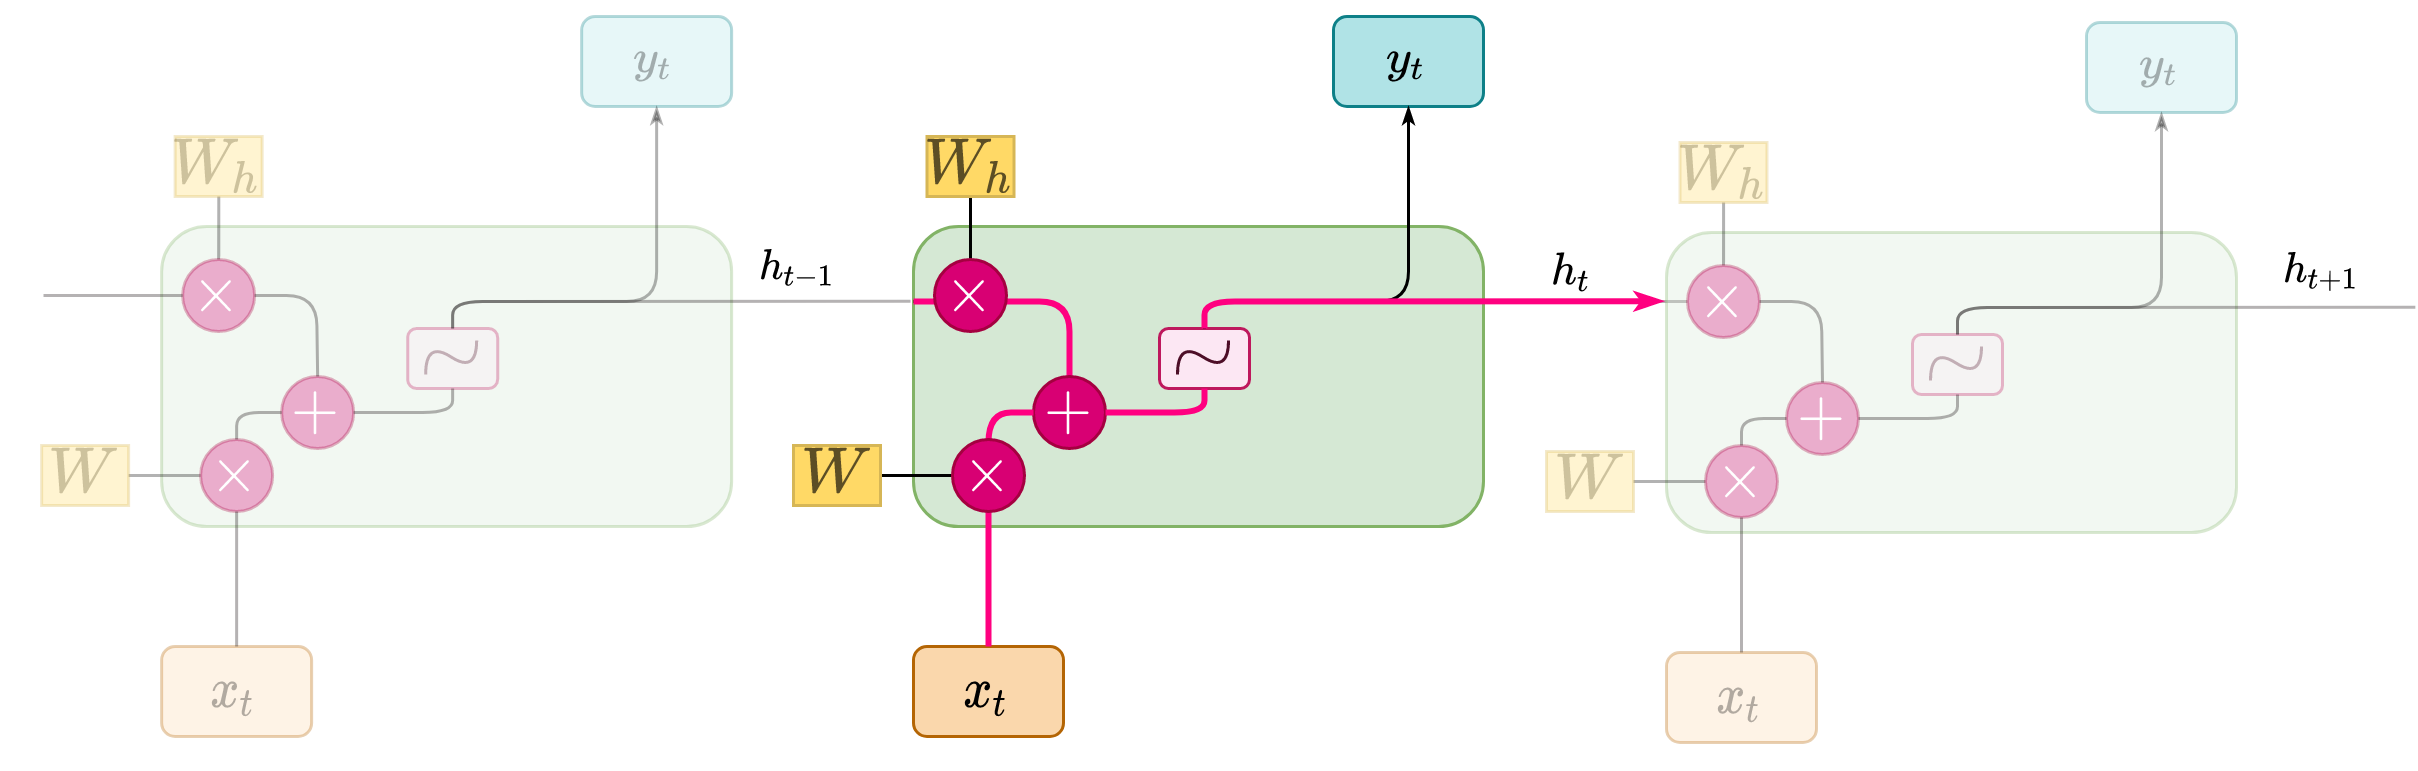
\includegraphics[width=14cm]{images/state-of-art/rnn/standard-rnn.png}
    \caption{Funcionamiento de una RNN}
\end{figure}
 
 Por cada iteración la presencia de información de anteriores $h$ va disminuyendo provocando el desvanecimiento del gradiente, concepto que se explicará posteriormente. Este flujo de información se puede ver mejor con el siguiente diagrama:

\begin{figure}[H]
    \centering
    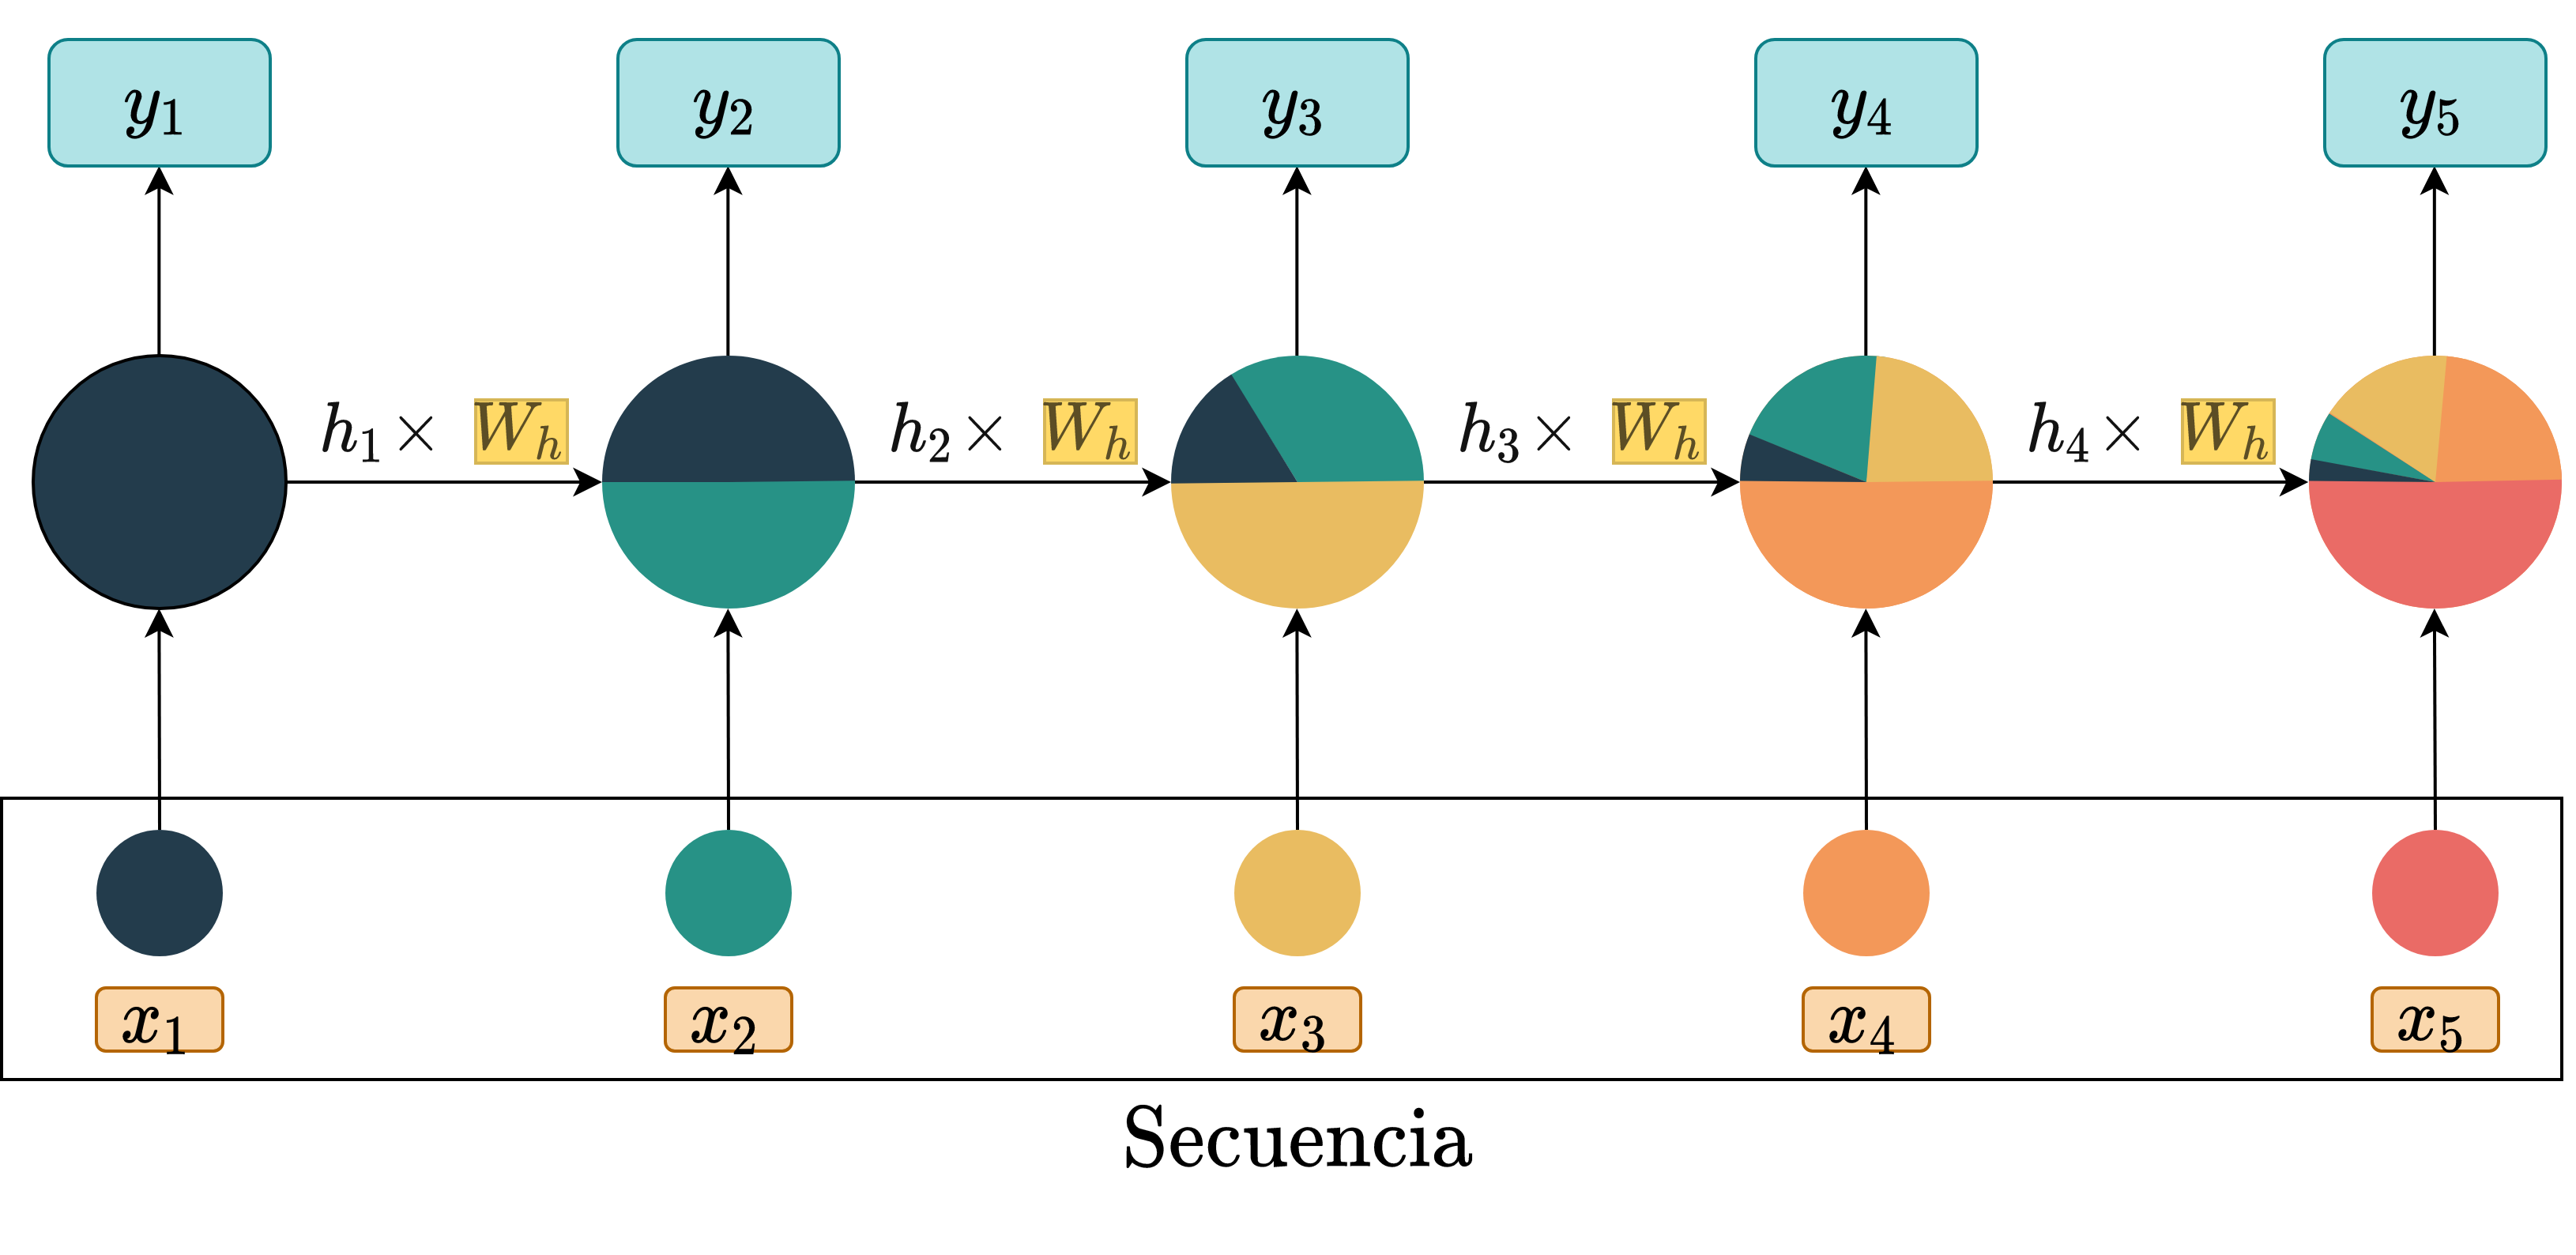
\includegraphics[width=11cm]{images/state-of-art/rnn/simple-rnn.png}
    \caption{Estructura de una capa recurrente}
    \label{fig:simple_rnn}
\end{figure}

Las capas recurrentes al igual que ocurre con las capas básicas de una red, tendrán asociado una matriz de pesos (aunque no tienen \textit{bias} $b$). Esta matriz será representada con $W_h$ dejando $W$ para matrices de pesos de capas básicas. Pueden existir múltiples capas recurrentes cada una con una matriz $W_h$ independiente cada una, por eso se hace uso del índice $RL_i$ como se ha explicado en la Figura \ref{fig:rnn-compact}.
\newline


El cálculo de $y$ es parecido al cálculo que se realiza en una red neuronal normal. Partiendo de la ecuación explicada en la Ecuación \ref{eqn:feedforward}:
\begin{equation}
    y = a(W^{L_l} \cdot (a(W^{L_{l-1}} \cdot ... \cdot (a(W^{L_1} \cdot x')^{L_1})) \text{ } ... \text{ } ^{L_{l-1}}))^{L_l}
\end{equation}

Simplificando este cálculo a una sola capa:
\begin{equation}
    \begin{split}
        z &= W^{L_l} \cdot y^{L_i} \\
        y &= a(z)
    \end{split}
\end{equation}

Si se trata de una capa recurrente, se ha de añadir un nuevo sumando a la operación, pero se quiere que siga teniendo las mismas propiedades de la función de activación, por lo que en realidad, lo que se va a modificar es el cálculo de $z$:
\begin{equation}
    \begin{split}
        z &= W^{L_l} \cdot y^{L_i} + W_h \cdot h \\
        y &= a(z)
    \end{split}
\end{equation}


Por ejemplo si se tiene una red recurrente formada por cinco capas, donde la primera y la tercera son capas recurrentes, el cálculo de $y$ final es el siguiente:
\begin{equation}
    y = a(W^{L_5} \cdot a(W^{L_4} \cdot a(W^{L_3} \cdot a(W^{L_2} \cdot a(W^{L_1} \cdot x' + W_h^{RL_1} \cdot h_1 ))^{L_2} + W_h^{RL_2} \cdot h_2)^{L_3})^{L_4})^{L_5}
\end{equation}


El cálculo de $z$ dependerá de si la capa recurrente es la primera:
\begin{equation}
    z^{L_1} = W^{L_1} \cdot x' + W_{h} \cdot h
\end{equation}

En otro caso, si la capa recurrente no es la primera:
\begin{equation}
    z^{L_i} = W^{L_i} \cdot y^{L_{i-1}} + W_{h} \cdot h
\end{equation}

